\documentclass{beamer}

\usepackage{multicol,graphicx}

\usetheme{Warsaw}
%\usecolortheme{beetle}

\title{Gettysburg Cemetery Dedication}
\author{Abraham Lincoln}
\institute{United States of America}
\date{19 Nov 1863}


\begin{document}



\begin{frame}
% you can use \titlepage or \maketitle to make beamer title page
\maketitle
\end{frame}

\begin{frame}
\frametitle{Outline}
\tableofcontents
\end{frame}


\begin{frame}
\frametitle{Agenda}
\section{Agenda}
\begin{itemize}
\item Met on battlefield (great)
\item Dedicate portion of field --- fitting!
\item Unfinished work (great tasks)
\end{itemize}
\end{frame}



\begin{frame}
\frametitle{Not on Agenda!}
\begin{itemize}
\item Dedicate
\item \pause Consecrate
\item \pause Hallow (in narrow sense)
\item \pause Add or detract
\item\pause  Note or remember what we say
\end{itemize}
\end{frame}



\begin{frame}
\frametitle{Key Objectives \& Success Factors}
\section{Review}
\begin{itemize}
\item What makes nation unique:
	\begin{itemize}
	\item Conceived in Liberty
	\item Men are equal
	\end{itemize}
\end{itemize}

\begin{block}{Shared vision:}
\begin{itemize}
\item New birth of freedom.
\item Gov't of/for/by the people.
\end{itemize}
\end{block}
\end{frame}

\begin{frame}
\frametitle{Organizational Overview}

\begin{center}
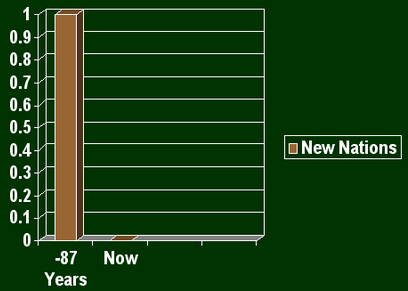
\includegraphics[scale=0.4]{gettysburg_graph}
\end{center}

\begin{block}{Four Score and Seven}
\begin{equation}
-(4 * 20 + 7) = -87
\end{equation}
\end{block}
\end{frame}


\begin{frame}
\frametitle{Summary}
\section{Summary}
\begin{columns}
\begin{column}{0.4\textwidth}
\begin{itemize}
\item New nation
\item Civil war
\item Dedicate field
\end{itemize}
\end{column}
\begin{column}{0.6\textwidth}
\begin{itemize}
\item Dedicated to unfinished work
\item New birth of freedom
\item Government not perish
\end{itemize}
\end{column}
\end{columns}
\end{frame}









\end{document}